\chapter{Theoretical framework}
\label{ch:marco}

\section{Convolutional neural networks}

A standard neural network consists of many simple, connected processors called neurons,
each producing a sequence of real-valued activations. Input neurons get activated through 
sensors perceiving the environment, other neurons get activated through weighted connections from previously
active neurons.

Learning is about finding specific weights that make the network exhibit desired behavior,
such as driving a car. Depending on the problem and how the neurons are connected, such behavior
may require long causal chains of computational stages, where each stage transforms 
the aggregate activation of the network. Deep Learning is an area of machine learning that tries to
replicate this behavior by increasing the number of stages \cite{schmidhuber2015deep}.
Figure \ref{fig:nnvscnn} shows the difference between regular NNs and deep NNs.

\begin{figure}
  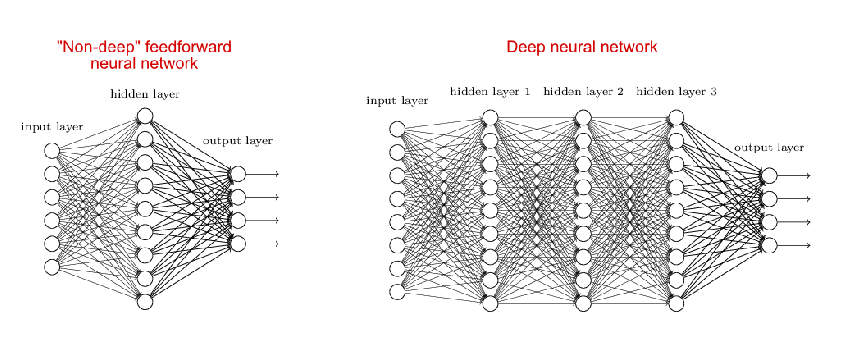
\includegraphics[width=\linewidth]{fig/nnvscnn.eps}
  \caption{Illustration of the difference between a regular neural network and a deep neural network \cite{nielsen2015neural}}
  \label{fig:nnvscnn}
\end{figure}

CNNs are part of deep learning, a type of neural network based on the 
visual system of mammals \cite{fukushima1980neocognitron}\cite{hubel1968receptive}.
A CNN is usually comprised of three types of layers: convolution, pooling and 
fully-connected \cite{karpathy2016cs231n}. There could also be normalization and activation phases.

\subsection{Convolution layer}

The most important layer in CNNs, as it represents the main operation done throughout the layers 
of the network and makes it possible to highlight features of the input image.
It is based on the convolution operation, defined as such:

\begin{equation} \label{eq:convorig}
  s(t)
  =
  (x*w)(t)
  =
  \sum_{a=-\infty}^{\infty} x(a)w(t-a)
\end{equation}

However, in CNNs the input image and output result are typically multidimensional
arrays with a defined size, which means that convolution must be implemented
as a discrete function. Assuming a two-dimensional input I and an applied two-dimensional filter (kernel)
the resulting operation is defined as following:

\begin{equation} \label{eq:convdiscr}
  S(i,j)
  =
  (K*I)(i,j)
  =
  \sum_{m}\sum_{n} I(i-m,i-n)K(m,n)
\end{equation}

If the kernels are smaller than the input image, each of them will only filter a 
specific window of the image at a time
while sliding this window to cover the full image, generating an activation map. 
Also, because the images are color images,
the input will be a three-dimensional matrix which can be transformed (flattened 
and rearranged) and processed as a matrix multiplication
following the process found on \cite{suda}.

This sliding window will allow to cover the whole input image by moving a certain number of pixels after every operation, this number is called stride.
Also, because the filter operates on every pixel of the window and to ensure a proper output size, a border of ceros could be added to the input
image with a specific width, called zero-padding \cite{karpathy2016cs231n}. The last parameter to take into account is the number of kernels to use per layer.
Another relevant term is a feature map, which is any output of the layers conforming the CNN \cite{Goodfellow-et-al-2016}.

Suda et al. define the equation that describes the output of a single neuron convolution operation applied to a specific (x,y) position on 
the input matrix as:

\begin{equation} \label{eq:convsuda}
  out(f_o,x,y)
  =
  \sum_{f_i=0}^{N_{if}}\sum_{k_x=0}^{K}\sum_{k_y}^{K} wt(f_o,f_i,k_x,k_y)in(f_i,x+k_x,y+k_y)
\end{equation}

Where $out(f_o,x,y)$ and $in(fi,x,y)$ represent the neurons at location
$(x,y)$ in the feature maps $f_o$ and $f_i$, respectively and 
$wt(f_o,f_i,k_x,k_y)$ are
the weights at position $(k_x,k_y)$ that gets convolved with input
feature map $f_i$ to get the output feature map $f_o$. This is done 
for all $N_{if}$ input features \cite{suda}.

\subsection{Pooling Layer}

A pooling function replaces the output of the NN at a certain 
location with a summary of the nearby outputs. For example, 
the max pooling \cite{zhou1988computation} operation reports the maximum 
output within a rectangular neighborhood. The objective is to discard
unnecessary details in the input matrix and preserving the important information.

Just like convolution, a sliding window is used and the pooling
operation is performed for each movement of the window. This process
reduces the output size (downsampling) \cite{karpathy2016cs231n}.

\subsection{Fully-connected Layer}

A fully-connected layer is similar to convolution with the difference being
that a convolution layer is connected only to a local region of the input matrix, 
while a fully-connected one operates over every activation in the previous layer.
Their objective is to take every feature found by the other layers and classify
them depending on the objects the CNN is trying to find, that is why they need
all information gathered by the previous layers. For this reason, fully-connected
layers are generally found at the end of the neural network architecture.

\subsection{Normalization}\label{theorylrn}

A normalization layer is common in CNN implementations to speed up convergence, accelerating
the process of getting the correct answer when training and evaluating.
A common form of normalization is local response normalization (LRN), defined
using the equation \ref{eq:lrnalex}, found on Krizhevsky's paper \cite{krizhevsky2012imagenet}.

\begin{equation} \label{eq:lrnalex}
  out(f_o,x,y)
  =
  \frac{in(f_o,x,y)}
  {\left(k+\alpha\sum_{f_i=max(0,i-n/2)}^{min(N-1,i+n/2)}in^2(f_i,x,y)\right)^\beta}
\end{equation}

$\alpha$, $\beta$, {\textit{k}}
and \textit{n}
are constants determined by a validation set,
while \textit{N}
is the amount of neurons per layer.

\subsection{Examples of CNN architectures}

One of the first successful CNN was LeNet, which was used for number detection
and classification on zip codes, digits and more. It consisted of three convolution
layers, two subsampling layers similar to pooling and one single fully-connected
layer at the end \cite{lecun1998gradient}.

VGG is another successful CNN which features up to 16 convolution layers, as well
as using max-pooling and fully-connected layers \cite{simonyan2014very}. It shows
that increasing the depth of conventional CNNs is enough to achieve the necessary
performance needed for large-scale image classification.

One of the most import CNNs developed in recent years is the one developed by 
Alex Krizhevsky, Ilya Sutskever and Geoff Hinton. Known as AlexNet, it innovated
by stacking convolutional layers and increasing the depth of the CNN \cite{krizhevsky2012imagenet}. 
This project uses a partially modified version of AlexNet.

%-----

\section{Approximate computing}

Approximate computing is a paradigm that tries to take advantage of the fact that
many applications can still work properly even with errors being introduced, be them
manually or by accident. Chippa et al. \cite{chippa2013analysis} show that current world
applications are error-resilient, meaning that they can withstand the introduction of errors
while having meaningful outputs.

Approximate computing can be applied to many fields of computer programming and organization stack.
There can be approximate programming languages that introduce imprecise algorithms, 
to approximate compilers that generate imprecise but fast machine code.
There are also approximate computer architectures, going down into approximate memory and hardware that allow for 
less energy consumption and better performance \cite{surveyqu}.

\subsection{Approximate hardware definition}

Using approximate hardware is a good approach when having access to transistor-level definition.
There have been efforts that try to design approximate logical units \cite{kim2013energy}\cite{ye2013reconfiguration}
which could improve the energy levels of existing arithmetic units. But this approach is 
not viable when working with FPGAs as we can only change the functionality of the hardware
instead of its electric properties or composition.

For high-level synthesis, introducing errors must be done partially, as not every
part of the hardware can be imprecise. Some of the most important approaches have been:

\begin{itemize}
  \item Finding the minimum area under a given error rate constraint. Shin and Gupta
  show that an error of at least 1\% can lead to reductions of up to 9\% in the area
  utilized by the design \cite{shin2010approximate}.
  \item Using an iterative process to improve the synthesis by taking into account
  the error magnitude \cite{miao2013approximate}.
  \item SALSA. A methodology to allow for better control of the quality constraints
  and transforming the approximate hardware synthesis problem into a regular synthesis
  problem \cite{venkataramani2012salsa}. There is also an extension to it called ASLAN
  that works for sequential circuits \cite{ranjan2014aslan}.
  \item Axilog is an extension to Verilog that allows the designer to choose which parts
  of the design can be approximate or exact \cite{yazdanbakhsh2015axilog}.
  \item Working on fixed point arithmetic can be analyzed and bitwidth optimizations
  applied for precise control of the accuracy of the output \cite{li2015joint}.
\end{itemize}

\subsection{Approximate neural networks}

Agrawal et al. demonstrate that DNNs are resilient to numerical errors
from approximate computing. By removing random computations on the convolution layers 
and using single-precision floating-point number representation, they achieved an error
of about 18\% \cite{approximatecomp}.

Moreau et al. created a neural accelerator, called SNNAP, that approximates the filter functions and
communications between each component within a FPGA-based application \cite{moreau2015snnap}. This can be used
to generate approximate kernels adapting the SNNAP replacements to OpenCL and the neural network
definition.

Another technique is the use of fixed-point arithmetic with less bitwidth for the data being
computed inside the neural network. Wang et al. showed that a neural network can be 
trained using 8-bit floating point numbers without reduced accuracy on the final result \cite{wang2018training}.
Using fixed-point arithmetic on different layers could be used to change the precision of
each of the layers, adjusting them and experimenting to obtain the best results energywise
while trying to maintain an accepted output.

Most of the current CNNs have a lot of layers for fine tuning the output classification.
Simonyan presents various CNN models with different number of layers, finally setting for
16 convolution layers and 3 fully-connected layers \cite{simonyan2014very}. Looking at the 
results, the other configurations with less layers could be used in order to improve performance,
reduce implementation area and reduce energy consumption, while the error is only
reduced a little after many layers are included.

\subsection{Approximate FPGA implementations}

Lopes et al. explore the opportunities to explore on playing with the number of iterations
on FPGA computations \cite{roldao2009more}. By using iterative solutions to linear systems, 
the final precision of each calculation and the accuracy can 
be adjusted by executing less or more iterations.
This can be used in conjunction with the operations defined by the neural network kernels 
to finely control the precision of each layer or the whole network.

As already mentioned, Moreau's neural accelerator can be used to approximate functions implemented
on FPGAs. This approach allows to create a specific implementation that does not interfere
with other techniques. There is also the framework introduced by Sampson \cite{sampson2015accept},
which enables programmers to manually adjust the approximation while providing automation
for the process. Sampson showed good results using the framework on a SoC with an FPGA as an
approximate accelerator.

There can also be optimization on the arithmetic operations defined on each of the functions
to be run on the FPGA. Approximate multipliers can be used to accelerate the performance
of matrix multiplications, convolution and other operations that use multiplications
\cite{ullah2018smapproxlib}. This can be improved upon by ways of memoization, a technique
that stores a cache for expensive calculations and returns this cache whenever those
calculations are repeated. Using memoization has already been proved to work on FPGA
implementations \cite{sinha2016low} and, while it comes with a small cost on area, it can be used to speed
up calculations by large amounts.

\section{\intelOCLnos}

The use of heterogeneous devices, from general-purpose GPUs to FPGAS, to execute 
machine learning algorithms and neural networks
is of big interest in the current world. There are current efforts to bring
all types of devices together by taking
advantage of each device strengths \cite{abadi2016tensorflow}.

OpenCL is a framework developed by Apple Inc. that allows for a seamless
programming experience for heterogeneous devices. OpenCL is based on 
the C++ 14, including most constructs from C++ in order to work as a
clone of it. This allows high-level programmers to develop applications
that can be run on different platforms without having to create new code
for any new platform.

\intelOCLnos is a development environment that allows the creation of
synthesizable kernels, blocks of code that can be executed within the FPGA.
Because of the high-level focus of OpenCL, it can be used to design in short
time big application such as CNNs. As for its effectiveness, it has been
demonstrated that using OpenCL instead of low-level languages such as Verilog
does not yield bad performance results, at the cost of a little more memory
usage \cite{abdelfattah2014gzip}.

OpenCL requires two different pieces of code: a host code and a device code. The
host code is in charge of determining the device on which the main computation is
going to run, prepare the data to be processed and, in the case of FPGAs, run the 
programming process in order to start the execution. The device code is the
code that is programmed into the FPGA and represents the hardware execution process.

Suda et al. \cite{suda} implement an FPGA accelerator for CNNs. They take advantage
of the parallelism offered by OpenCL in order to set vectorization and 
loop unrolling factors as to have better control of the actual implementation
on the FPGA. Also, Suda's implementation applies convolution using
matrix multiplication, achieving good performance on these layers. Suda
uses AlexNet and VGG to benchmark its results, finding that it can be
significantly better than the CPU time.

Wang et al. \cite{pipecnn} created a reconfigurable accelerator for CNNs
based on OpenCL. This implementation features OpenCL's extended channel support 
on FPGAs enabling communication between layers without using onboard memory, allowing
for reduced memory usage and faster communication between layers.
This work demonstrates high performance and shows the low energy consumption
of FPGAs. It also uses AlexNet and VGG to get its results.